%%%%%%%%%%%%%%%%%%%%%%%%%%%%%%%%%%%%%%%%%%%%%%%%%%%%%%%%%%%%%%%%%%%%%%%%%%%%%%%

\chapter{TRABALHOS CORRELATOS}\label{ch:corr}

Nessa seção são apresentados os trabalhos correlatos a essa proposta, que podem ser divididos em duas seções: as soluções de \textit{Big Data} de outros operadores, e os algoritmos existentes de construção do cubo de dados com alta dimensionalidade.

\section{Dados da operação}\label{ch:corr:data}

A tabela~\ref{table:bigdatasattypes} mostra os tipos de dados relevantes para a operação, a sua origem e o seu formato esperado.
Essa tabela considera apenas dados considerados como telemetria do próprio satélite, ou dados advindos de terceiros.

\begin{table}[!ht]
	\begin{center}
		\caption{Dados de Operação}\label{table:bigdatasattypes}
		\begin{tabular}{|c|C{5cm}|c|}
			\hline
			\bfseries Tipo de Dado         & \bfseries Origem           & \bfseries Formato      \\
			\hline
			Sensores de bordo              & Equipamentos no satélite   & Tabelas, CSV           \\
			\hline
			Registros do Computador        & Computador de Bordo        & Texto (\textit{Logs})  \\
			\hline
			Multimídia                     & Câmeras                    & MP4, JPG, RAW          \\
			\hline
			Parâmetros orbitais            & Operação, Rastreio         & TLE, texto, tabelas    \\
			\hline
			Documentação associada         & Operadores, engenharia     & Texto (Word, Excel)    \\
			\hline
			Clima Espacial                 & Sensores no solo ou espaço & Texto, tabelas, avisos \\
			\hline
			\textit{Situational Awareness} & Radares, US-STRACOM, etc   & Texto, tabelas, avisos \\
			\hline
		\end{tabular}
	\end{center}
	\FONTE{Adaptado de~\cite{zhangBigDataFramework2017}}
\end{table}

Para este trabalho, apenas os dados vindos de sensores de bordo serão considerados.
Os outros dados nesta tabela poderiam ser considerados para uma \textit{Data Warehouse} mais completa, porém estão fora do escopo desta proposta.

\subsection{Fluxo dos Dados}\label{ch:corr:dataflow}

Baseado nos trabalhos correlatos e nos dados levantados, a figura~\ref{fig:bigdataflow} demonstra o fluxo de dados esperado de uma arquitetura de \textit{Big Data} para a operação de satélites.

\begin{figure}[ht]
	\caption{Fluxo de dados em uma arquitetura de \textit{Big Data}}\label{fig:bigdataflow}
	\vspace{6mm}
	\begin{center}
		\resizebox{15cm}{!}{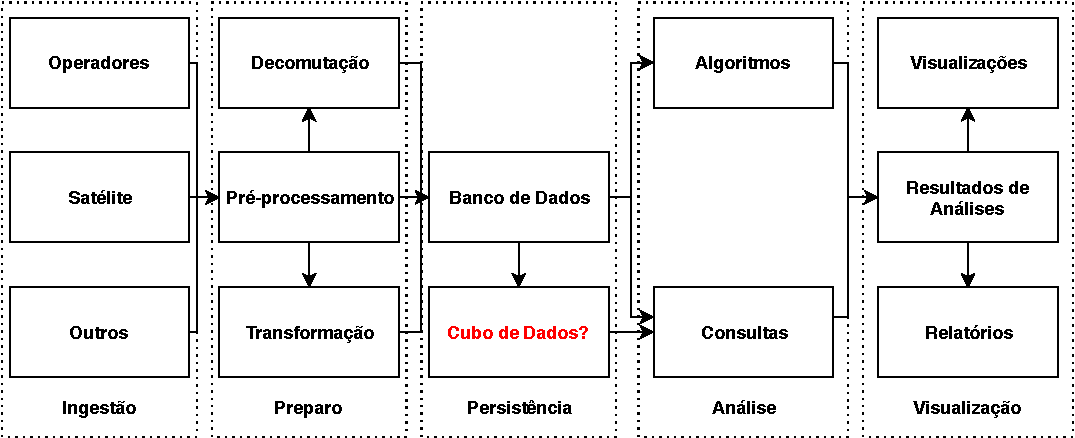
\includegraphics{Figuras/BigDataFlow.pdf}}
	\end{center}
	\vspace{2mm}
	\legenda{}
	\FONTE{Adaptado de~\cite{zhangBigDataFramework2017}}.
\end{figure}

Este fluxo está separado em cinco etapas que vão desde a origem dos dados até o seu resultado de análise, e este trabalho visa apenas mapear qual seria esse fluxo baseado nos trabalhos correlatos.
Cada uma das etapas está detalhada a seguir:

\begin{itemize}
	\item \textbf{Ingestão}: onde os dados serão coletados na sua fonte (satélites, sensores no solo, outras fontes, etc).
	      Essa etapa trata de \textbf{onde} estão os dados e \textbf{como} coletá-los, bem como \textbf{quais} são os dados importantes de serem coletados.
	      A ``fonte'' aqui pode ser um serviço de terceiros, dentro da própria instituição ou disponível de outra forma.
	\item \textbf{Preparo}: os dados relevantes são selecionados, e transformações são realizadas para inserir os mesmos na base de dados.
	      Essa etapa trata do formato específico dos dados, realizando operações de limpeza, verificação da qualidade e da relevância para a análise, entre outras.
	      O seu objetivo é garantir que os dados tem qualidade, relevância, e estão no formato adequado para a base de dados.
	\item \textbf{Persistência}: após o devido processamento, os dados de alta qualidade são guardados em uma base de dados, de onde ficarão disponíveis para a análise.
	      Nessa etapa um banco de dados é utilizado, tratando apenas em como esses dados estão guardados e como eles serão disponibilizados para as consultas e execução de algoritmos.
	\item \textbf{Análise}: nesta etapa são executadas as consultas e os algoritmos de interesse para a análise.
	      Podem ser desde consultas simples (``qual era o valor da telemetria X durante a passagem Y?''), a execução de algoritmos complexos (``preveja os valores da telemetria X para a próxima passagem'').
	\item \textbf{Visualização}: os resultados das consultas e algoritmos são visualizados.
	      Podem conter desde gráficos simples, como um histograma de uma telemetria, a relatórios complexos de um subsistema/satélite, bem como resultados de algoritmos.
\end{itemize}

Os trabalhos de~\cite{zhangBigDataFramework2017},~\cite{mateikUsingBigData2017} e~\cite{boussoufBigDataBased2018} definem esse processo mais claramente dentre os trabalhos apresentados.

\section{Análise de Dados em Outros Operadores de Satélite}\label{ch:corr:ops}

A tabela~\ref{table:bigdataoperators} mostra uma revisão feita em artigos recentes sobre os operadores de satélite e quais tecnologias eles estão utilizando para atingir objetivos semelhantes, principalmente com o uso de \textit{Big Data}.

\begin{table}[htbp]
	\begin{center}
		\caption{Operadores de Satélite e Arquiteturas de Big Data}\label{table:bigdataoperators}
		\begin{tabular}{|C{8em}|C{6em}|c|C{10em}|}
			\hline
			\bfseries Referência                           & \bfseries Operador & \bfseries Ferramenta & \bfseries Tecnologias                                                                \\
			\hline
			\cite{adamskiDataAnalyticsLarge2016}           & L3 (EUA)           & InControl            & Hadoop, Spark, HBase, MongoDB, Cassandra, Amazon AWS                                 \\
			\hline
			\cite{boussoufBigDataBased2018}                & Airbus             & Dynaworks            & Hadoop, Spark, HDFS, HBase, PARQUET, HIVE                                            \\
			\hline
			\cite{schulsterCHARTingFutureOffline2018}      & EUMETSAT           & CHART                & MATLAB, MySQL, Oracle                                                                \\
			\hline
			\cite{zhangBigDataFramework2017}               & SISET (China)      & -                    & Hadoop, HDFS, PostgreSQL, MongoDB, Logstash, Kibana, ElasticSearch, Kafka, MapReduce \\
			\hline
			\cite{yvernesCopernicusGroundSegment2018}      & Telespazio France  & PDGS                 & OLAP (DataCube), Saiku, Pentaho, Jaspersoft OLAP                                     \\
			\hline
			\cite{dischnerCYGNSSMOCMeeting2016}            & SwRI + NOAA        & CYGNSS MOC           & SFTP, -                                                                              \\
			\hline
			\cite{edwardsDealingBigData2018}               & EUMETSAT           & MASIF                & FTP, RESTful service, JMS Messague Queue, PostgreSQL                                 \\
			\hline
			\cite{evansDataMiningDrastically2016}          & S.A.T.E + ESA/ESOC & -                    & Java, CSV                                                                            \\
			\hline
			\cite{fenManagementOperationCommunication2016} & CSMT (China)       & -                    & não menciona as tecnologias                                                          \\
			\hline
			\cite{trollopeAnalysisAutomatedTechniques2018} & EUMETSAT           & CHART                & algoritmos ad-hoc, estudo de caso                                                    \\
			\hline
			\cite{gillesFlyingLargeConstellations2016}     & L-3                & InControl            & Amazon EC2, LXC, Nagios                                                              \\
			%\hline
			%\cite{highsmithSpaceLaunchSystem2015} & Boeing + NASA & - & lançadores, não é o foco da arquitetura \\
			\hline
			\cite{hennionBigdataSatelliteYearly2018}       & Thales Alenia      & AGYR                 & Logstash, Kafka, InfluxDB, ElasticSearch, Kibana, Grafana                            \\
			\hline
			\cite{mateikUsingBigData2017}                  & Stinger, NASA      & -                    & Logstash, ElasticSearch, Kibana, HDF5, CSV, R, Python, AWS, Excel                    \\
			\hline
			\cite{fernandezTelemetryAnomalyDetection2017}  & NASA               & MARTE                & R, CSV, ad-hoc                                                                       \\
			\hline
		\end{tabular}
	\end{center}
	\FONTE{Produção do autor.}
\end{table}

Os objetivos em comum desses trabalhos são facilitar as atividades dos operadores por meio de algoritmos de detecção de anomalias e de verificação dos limites nos valores das telemetrias.
Alguns dos operadores dessa lista estão responsáveis pela operação de constelações de satélites complexos, como constelações de sensoriamento remoto, que faz necessário um certo nível de automação ou a operação contínua teria um custo inviável.

Nesses trabalhos, o uso dessas tecnologias é apenas para os operadores de satélite, pois em nenhum desses trabalhos eles estão na mesma estrutura de ingestão dos dados da carga útil, mesmo utilizando as mesmas tecnologias, como demonstrado em~\cite{mateikUsingBigData2017} e~\cite{adamskiDataAnalyticsLarge2016}.

Alguns desses trabalhos não utilizam de estruturas completas que seguem um fluxo de dados, como é o caso de~\cite{fernandezTelemetryAnomalyDetection2017} e~\cite{trollopeAnalysisAutomatedTechniques2018} que utilizam de \textit{scripts} feitos de forma \textit{ad-hoc}, não mostrando uma visão da arquitetura completa do fluxo de dados e apenas a ferramenta utilizada para análise pontual.

O trabalho de~\cite{yvernesCopernicusGroundSegment2018} utiliza de estratégias OLAP e do cubo de dados, tendo utilizado uma modelagem dimensional para a operação de uma constelação de satélites, porém esse trabalho menciona apenas em alto nível a modelagem utilizada, e menciona que o trabalho foi somente na parte da modelagem dimensional e integração dos dados utilizando ferramentas já existentes.

\subsection{Análise de Dados no INPE}\label{ch:corr:inpe}

O INPE já realiza análise de dados em outros departamentos, inclusive sobre as telemetrias de satélite.
Os operadores devem monitorar os valores das telemetrias e informar a engenharia caso apareça algum problema que não pôde ser corrigido~\cite{TominagaFerrAmbr:2017:CoSaTe}.
Um exemplo está no trabalho~\cite{Magalhaes:2012:EsAvTe}, feito sobre uma falha no satélite CBERS-2, onde o modelo proposto visa melhorar o conhecimento sobre avalanche térmica nas baterias para impedir que isso aconteça novamente em outros satélites.
A motivação principal dos trabalhos da tabela~\ref{table:bigdataoperators} era a detecção de anomalias, que teve alguns algoritmos estudados em~\cite{AzevedoAmbrViei::EsSoTe}.

Outros setores, utilizam a análise de dados vindos da carga útil do satélite ou de agentes externos ao INPE, como dados de sensoriamento remoto, cuja análise não é trivial e também estão classificados como \textit{Big Data}.
~\citeonline{monteiroFRAMEWORKTRAJECTORYDATA2017} utilizam de conceitos de Big Data para análise de trajetórias de objetos;~\citeonline{ramosDistributedSystemsPerformance2016} demonstram o uso de softwares como o Hadoop para a análise de dados do clima espacial, com uma arquitetura relacionada as arquiteturas revisadas na seção anterior; e~\citeonline{SimoesCamaQuei:2018:DaAnMa} mostra uma arquitetura que utiliza de cubo de dados para a análise de séries temporais no sensoriamento remoto.

\section{Computação do cubo de dados}\label{ch:corr:cube}

A computação seletiva do cubo de dados possui muitos algoritmos diferentes implementados, porém eles possuem dificuldades no trato de dados com muitas dimensões e no uso limitado da memória~\cite{hanDataMiningConcepts2011}.

O \textit{FragCubing}~\cite{liHighdimensionalOLAPMinimal2004} apresenta o conceito de \textit{cube shells}, onde subcubos com poucas dimensões (de 3 a 5 neste exemplo) são calculados utilizando de índices invertidos, que funcionam apenas utilizando memória principal.
A ideia principal é decompor o cubo original em fragmentos que podem ser reunidos eficientemente para responder uma consulta multidimensional.

Precursor para o computação distribuída do cubo,~\cite{dokaBrownDwarfFullydistributed2011} apresenta o \textit{Brown Dwarf}, um sistema \textit{Peer-to-Peer} que permite atualização das células, desenhado para diminuir a redundância em cubos distribuídos.

O \textit{PopUp-Cubing} é apresentado em~\cite{heinePopUpCubingAlgorithmEfficiently2017}, que utiliza de icebergs para lidar com dados em formato de \textit{stream}, obtendo resultados superiores ao FTL e \textit{Star-Cubing}.
Este trabalho é de interesse especial por utilizar de dados de \textit{stream}, que permitiriam resultados parecidos com tempo real, que são mais parecidos com os dados disponíveis para a operação de satélites, porém este cenário não será abordado neste trabalho.

Com foco em \textit{Big Data} e utilizando como base o esquema \textit{MapReduce},~\cite{wangScalableDataCube2013} apresenta o algoritmo \textit{HaCube} para computação do cubo em paralelo.
Este trabalho apresenta um balanço entre computação do cubo em paralelo por vários nós de \textit{MapReduce}, que permite algumas atualizações e computação incremental de medidas.
Devido a própria natureza distribuída, ele precisa de mecanismos de tolerância a falha, e também os testes foram executados com no máximo apenas 5 dimensões, porém com até 2,4 bilhões de tuplas.
Ainda na linha do \textit{MapReduce},~\cite{yangHolisticAlgebraicData2017} demonstra a computação de medidas holísticas apresentando o \textit{Multi-RegionCube}, porém realizando menos testes que o \textit{HaCube}.

Em~\cite{zhaoClosedFragShellsCubing2018} é apresentado o \textit{Closed Frag-Shells Cubing}, que utiliza de uma combinação da abordagem de cubos fechados com a abordagem \textit{Shell fragments}, obtendo resultados melhores que a aplicação de cada uma delas separadamente.
Essa abordagem utiliza de índices \textit{bitmap} e índices invertidos, sendo que lidam com dados altamente dimensionais e sem uma hierarquia de forma similar ao necessário neste trabalho.

\textit{qCube}~\cite{silvaQCubeEfficientIntegration2013} estende a abordagem \textit{FragCubing} para permitir consultas sobre intervalos de valor, estendendo os operadores de consultas clássicas em cubo de dados além do operador de igualdade.

\textit{HFrag}~\cite{silvaHybridMemoryData2015} apresenta o uso de memória externa na computação dos índices invertidos, utilizando de um sistema híbrido de memória para armazenar as partições do cubo tanto na memória principal quanto na secundária, com os valores mais frequentes sendo armazenados na memória principal e os valores menos frequentes na memória secundária.

A abordagem \textit{Hybrid Inverted Cubing} (HIC)~\cite{silvaComputingBIGData2016} estende a abordagem \textit{HFrag} com o parâmetro de frequência acumulada crítica, obtendo resultados melhores do que este nas mesmas consultas.

Destes trabalhos, o \textit{FragCubing} continua sendo um algoritmo robusto para a computação do cubo, com suas técnicas de índice invertido sendo utilizadas e ainda obtendo resultados adequados.
Porém,~\citeonline{liHighdimensionalOLAPMinimal2004} ilustram o impacto exponencial no consumo de memória nas diferentes abordagens de computação de cubos de dados usando apenas 12 dimensões, sendo que há uma saturação quando cubos com 20, 50 ou 100 dimensões são computados utilizando abordagens de cubos completos, cubos DWARF, MCG, cubos fechados ou quocientes~\cite{silva:2015:abordagensParaCubo}.

\subsection{FragCubing}\label{ch:corr:cube:frag}

O \textit{FragCubing}~\cite{liHighdimensionalOLAPMinimal2004} apresenta o conceito de inversão de tupla.
Cada tupla invertida $iT$ tem um valor de atributo, uma lista de identificadores da tupla (TIDs) e um conjunto de valores de medida.
Por exemplo, consideremos quatro tuplas: $t_1 = (tid_1, a_1, b_2, c_2, m_1)$, $t_2 = (tid_2, a_1, b_3, c_3, m_2)$, $t_3 = (tid_3, a_1, b_4, c_4, m_3)$, e $t4 = (tid_4, a_1, b_4, c_1, m_4)$.
Estas quatro tuplas geram oito tuplas invertidas: $iTa_1, iTb_2, iTb_3, iTb_4, iTc_1, iTc_2, iTc_3$ e $iTc_4$, demonstradas na figura~\ref{fig:fragexample}.

Para cada valor de atributo é construído uma lista de ocorrências, assim para $a_1$ temos $iTa_1 = (a_1, tid_1, tid_2, tid_3, tid_4, m_1, m_2, m_3, m_4)$ onde o valor de atributo a 1 está associado aos TIDs: $tid_1, tid_2, tid_3,$ e $tid_4$.
O identificador de tupla $tid_1$ tem o valor de medida $m_1$, $tid_2$ tem o valor de medida $m_2$, $tid_3$ tem o valor de medida $m_3$, e $tid_4$ possui o valor de medida $m_4$.
A consulta $q = (a_1, b_4, COUNT)$ pode ser respondida por $iTa_1 \cap iTb_4 = (a_1b_4, tid_3, tid_4, COUNT(m_3, m_4))$.
Em $q, iTa_1 \cap iTb_4$ indica os TIDs comuns em $iTa_1$ e $iTb_4$.

\begin{figure}[!htb]
	\caption{Exemplo de uma tabela dimensional e a respectiva lista de índices invertidos}\label{fig:fragexample}
	\vspace{2mm}
	\begin{center}
		\resizebox{15cm}{!}{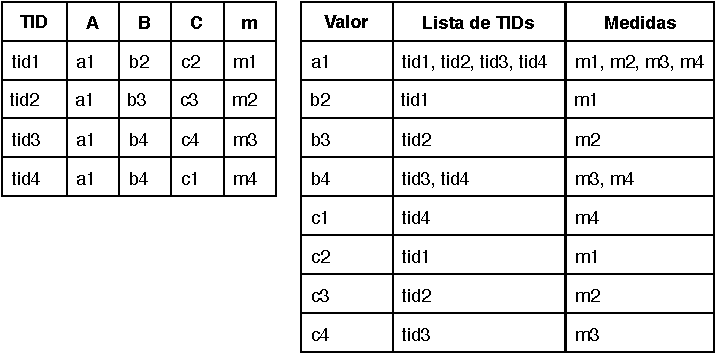
\includegraphics{Figuras/FragDrawing.pdf}}
	\end{center}
	\vspace{1mm}
	\legenda{}
	\FONTE{Produção do autor.}
\end{figure}

A complexidade da interseção é proporcional ao número de ocorrências de um valor de atributo, mais precisamente é igual ao tamanho da menor lista.
Neste exemplo, $iTb_2$ com um TID é a menor lista.
O número de TIDs associado a cada valor de atributo pode ser enorme, assim relações com dimensões de baixa cardinalidade e elevado número de tuplas necessitam de alta capacidade de processamento.
Listas de TIDs pequenas permitem que consultas sejam respondidas rapidamente, portanto relações com baixo \textit{skew} e alta cardinalidade são mais adequadas de serem computadas pela abordagem \textit{FragCubing}.

\textit{Skew} pode ser definido como o grau de uniformidade dos valores de atributos numa relação, sendo que \textit{skew} zero indica relação com valores de atributos uniformemente distribuídos, e quanto maior o \textit{skew} menos uniformemente distribuída a relação se encontra.
%Neste sentido, abordagens como \textit{FragCubing}, que fazem uso apenas de memória principal (\textit{RAM}), normalmente não conseguem computar cubos com alta dimensionalidade, cardinalidade e elevado número de tuplas eficientemente, pois extrapolam a memória existente e necessitam operações de swap do sistema operacional.

